\chapter[FM - Modulation and Demodulation using PLL]{FM - Modulation and Demodulation using PLL}
\section*{Aim}
To implement FM modulation and demodulation circuits using PLL IC CD4046
\section*{Theory}
CD 4046 is an analog Phase Locked Loop IC, whose characteristics and features are discussed in Appendix \ref{4046}. This IC can be used for FM modulation and demodulation.
\subsection*{FM Modulation}

The VCO part of the PLL may be used for the frequency modulation of the carrier. In a VCO, the output frequency is proportional to the control volatge input. In the absance of control voltage, the free running frequency is determined by the supply voltage $V_{CC}$, the externally connected resistances $R_1$ and $R_2$ and the capacitance C. The free running frequency $f_0$ is given by 
\begin{equation}
\label{f0}
f_0=\frac{0.16\ X\ \frac{V_{CC}}{2} }{R_1.C}+\frac{1}{R_2.C}
\end{equation}

The VCO in free running mode is the carrier generator. The carrier frequency is $f_0$.
 The control input of the VCO is clamped at a voltage $\frac{V_{cc}}{2}$. The modulating signal voltage which is less than $\frac{V_{cc}}{2}$  is applied at this pin through a capacitor. This results in variation in the frequency of oscillation of the VCO, which is the frequency modulated signal.

\subsection*{FM Demodulation}
Another PLL IC has to be used for FM demodulation. The VCO part of this IC is configured for the same free running frequency as that of the modulator IC. 

One of the  phase detector input is fed with the modulated FM signal and the other input of the phase detector is fed with the VCO output after filtering out high frequency componens. The phase variation between the two will be corresponding to the message which was used for modulation. The PD output is passed through an emitter follower internally to the demodulated output pin. The output from this pin may  contain high frequency ripples which may be eliminated by proper filtering to obtain the actual message. 

 
\section*{Design}

Supply $V_{CC}=5V$ at pin-16 and ground pin-8 of both  PLL ICs.

\paragraph{Modulation}


\noindent Use a voltage divider network of two resistors with $ R=10\ k\Omega$  for clamping the control voltage input (pin-9) at $\frac{V_{cc}}{2}=\ 2.5V$. 


\noindent Give a message signal of frequency 1kHz and amplitude  $1\ V_{pp}$ at control voltage input (pin-9) throgh a capacitor of $C_1=\ 1\mu F$.


\noindent Select $R_1=\ 10\ k\Omega$ (pin-11),   $R_2=\ 100\ k\Omega$ (pin-12) and $C=\  0.002 \mu F$(between pin-6 and pin-7) so that free running frequency as per equation \ref{f0} is given by,

\begin{equation}
f_0 =\frac{(0.16 ). (2.5V)}{(10k\Omega).(0.002\mu F)}+\frac{1}{(100k\Omega).(0.002\mu F)}=20 kHz+5 kHz=25 kHz
%f_0=\frac{(0.16 ). (2.5V) }{(10k\Omega).(0.002\mu F)}+\frac{1}{(100k\Omega).(0.002\mu F)}
\end{equation}
 
\noindent The FM output is obtaned from $VCO_out$ (pin-4) of first PLL IC.

\paragraph{Demodulation}



\noindent Use the same $R_1$, $R_2$ and $C$ for the second PLL IC so that the free running frequency remains the same as that of the modulating IC. 
Feed the signal input pin of phase detector (pin-14) of the second IC with the FM signal. The other input of phase detector (pin-3) is fed with VCO output (pin-4).

\noindent The output from phase detector(pin-2)  is fed back to  VCO input (pin-9) through a low-pass filter with $R_3=10\ k\Omega$ and $C_1=0.01\ 0.01\mu F$. 

\noindent The demodulated output is obtained from the pin-10 by pulling down using a resistor $R_p=10 \ k\Omega$. It is then low pass filtered at $fc=1.5 kHz$ to eliminate higher order ripples.

\begin{equation}
f_c=\frac{1}{2\pi R_fC_f}=1.5kHz
\end{equation}
Choose $C_f=0.01\ \mu F$.  $\therefore \ R_f=\ 10 \ k\Omega$.
\section*{Circuit Diagram}

The circuit diagram for FM modulation and demodulation are shown in figure \ref{fmpllckt}.

\begin{sidewaysfigure}[ht]
    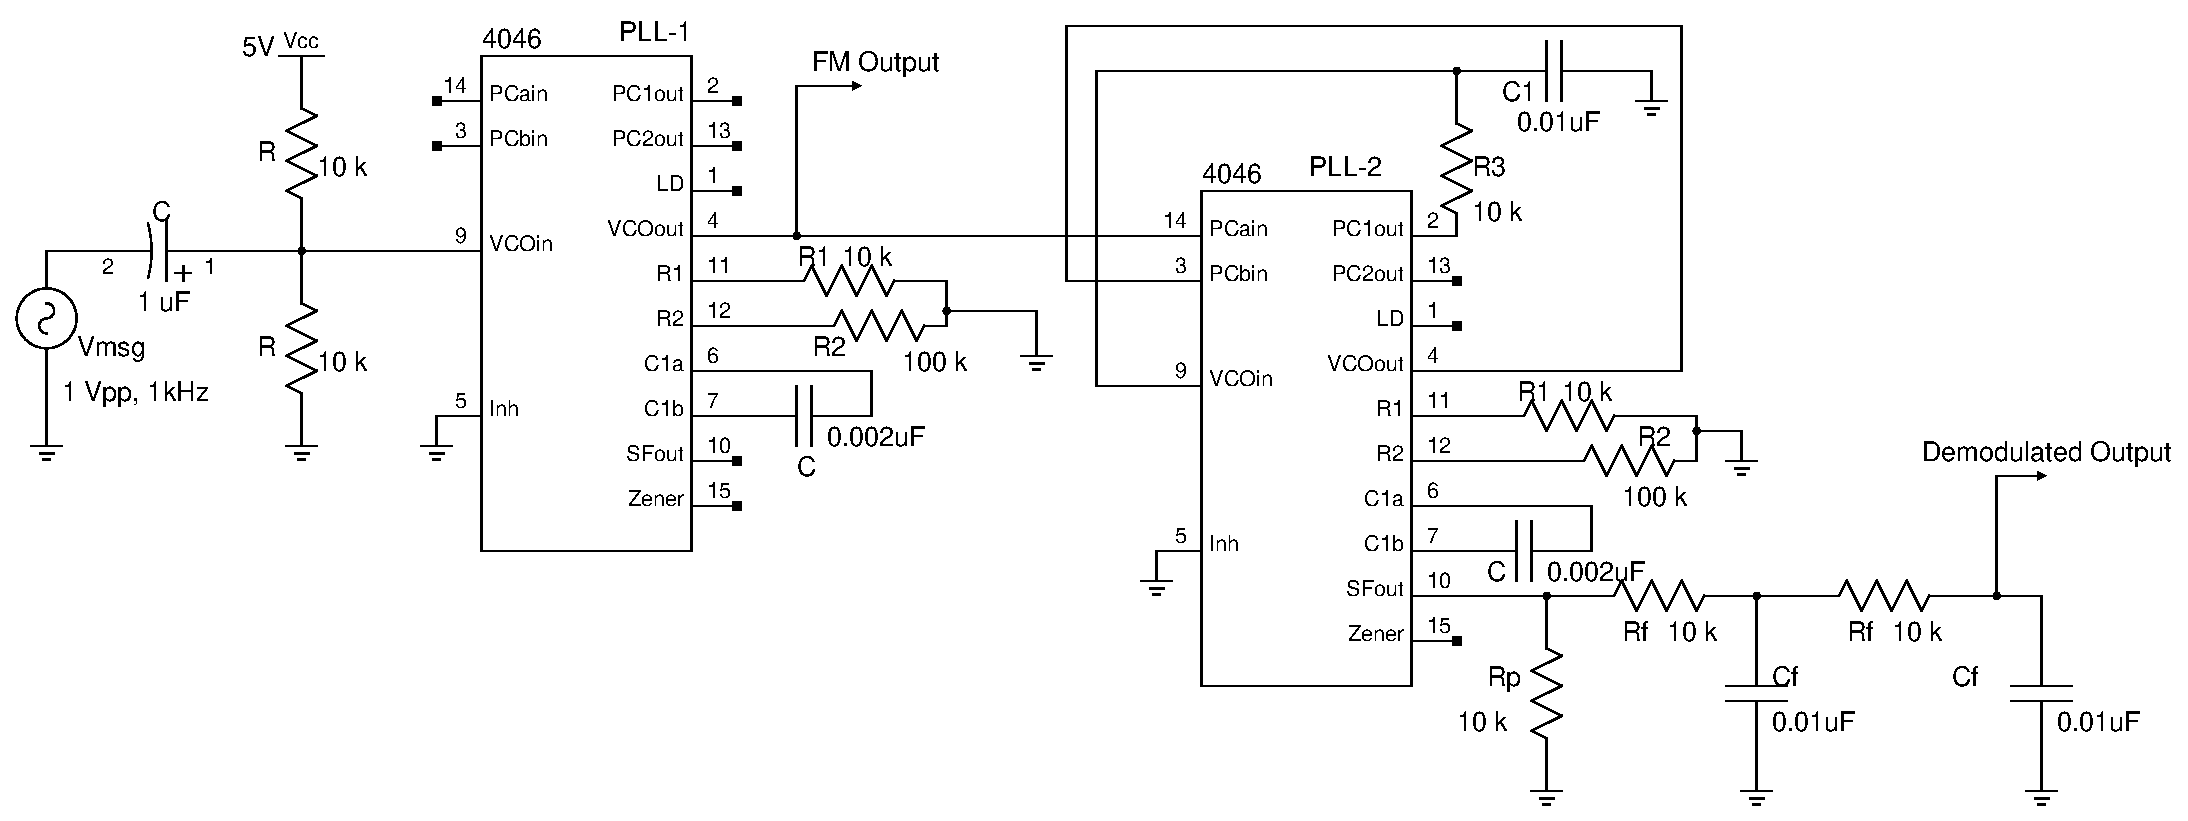
\includegraphics[scale=0.6]{fmpll.eps}
    \caption{Circuit for FM generation and detection using CD4046 PLL IC}
    \label{fmpllckt}
\end{sidewaysfigure}


\section*{Procedure}
\begin{itemize}
\item
Make connections as per the circuit digram.

\item
Provide dc supply and ground to the ICs.

\item
Observe the FM modulation and demodulation waveforms.

\item
Plot it on a graph sheet.
\end{itemize}
\section*{Observation}

Plot the message, carrier, modulated and demodulated waves on a graph sheet.
\section*{Result}
Implemented FM modulation and demodulation using PLL IC CD 4046.